Eine unit\"are Matrix besitzt einen oder mehere Eigenvektoren $|\psi\rangle$ mit zugeh\"origen Eigenwerten $e^{2\pi i \phi}$.
\begin{equation}
  U|\psi\rangle = e^{2\pi i \phi}|\psi\rangle
\end{equation}
Ein Zustand $|\psi\rangle$ ist gleich zu $e^{i\theta}|\psi\rangle$, bis auf der globalen Phase $e^{i\theta}$ \cite{nielsen_chuang_2010}. Die Bestimmung einer globalen Phase ist keine einfache Aufgabe, die Quanten-Phasensch\"atzung \textit{(quantum phase estimation)} kann diese Aufgabe jedoch l\"osen. Dies gilt unter der Bedingung, dass diese globale Phase die eines Eigenwertes ist. Die Schaltung der Quanten-Phasensch\"atzung (Abbildung \ref{fig:QPE}) wird auf zwei Quantenresgistern angewandt und wird aus zwei Teilen zusammengestellt. Das erste Quantenregister besteht aus $t$ Qubits die alle mit dem Basiszustand $|0\rangle$ initialisiert werden. Die Anzahl an Qubits f\"ur dieses Register wird nach der gew\"unschten Genauigkeit f\"ur die Sch\"atzung der Phase abh\"angig gemacht. Je gr\"o\ss er $t$ gew\"ahlt wird, desto gr\"o\ss er ist die Anzahl an Ziffern f\"ur die Sch\"atzung und auch die Wahrscheinlichkeit, dass die Phasensch\"atzung erfolgreich ist.
\begin{figure}[h]
  \centering
  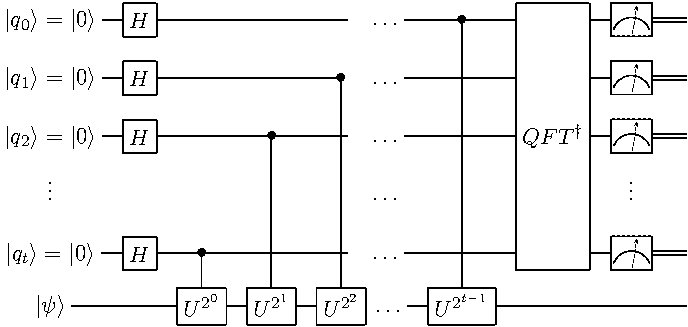
\includegraphics[width=1\textwidth]{figures/QPE.pdf}
  \caption{Allgemeine Schaltung der Quanten-Phasensch\"atzung}
  \label{fig:QPE}
\end{figure}
Das zweite Quantenregister ist der Eigenvektor $|\psi\rangle$, f\"ur dieses Register werden so viele Qubits genutzt wie f\"ur die Darstellung des Zustands ben\"otigt werden.\\\\
Im ersten Teil der Schaltung wird auf allen Qubits aus dem ersten Register eine Hadamard-Transformation ausgef\"uhrt. Daraufhin wird eine kontrollierte $U$-Transformation auf das zweite Register ausgef\"uhrt, bei diesem $U$-Gatter erh\"oht sich wie ersichtlich stetig die 2er Potenz. Im zweiten Teil der Schaltung wird auf das erste Register eine invertierte Quantum Fourier-Transformation angewandt. Dadurch endet das erste Register in folgenden Zustand \ref{eqn:QPE} \cite{nielsen_chuang_2010}.
\begin{equation}
  \label{eqn:QPE}
  \begin{aligned}
    &\frac{1}{2^{t/2}}\sum\limits_{k=0}^{2^t-1}e^{2\pi i\phi k}|k\rangle = \\
    &\frac{1}{2^{t/2}} \left(|0\rangle+e^{2\pi i 2^{t-1}\phi}|1\rangle\right)\otimes\left(|0\rangle+e^{2\pi i 2^{t-2}\phi}|1\rangle\right)\otimes\dots\otimes\left(|0\rangle+e^{2\pi i 2^{0}\phi}|1\rangle\right).
  \end{aligned}
\end{equation}
